\documentclass{article} % For LaTeX2e
\usepackage{format/nips14submit_e,times}
\usepackage{hyperref}
\usepackage{url}

% For figures
\usepackage{graphicx} % more modern
%\usepackage{epsfig} % less modern
\usepackage{subfigure} 

% For citations
\usepackage{natbib}

% For algorithms
\usepackage{algorithm}
\usepackage{algorithmic}

\usepackage{color}
\usepackage{preamble}
\definecolor{mydarkblue}{rgb}{0,0.08,0.45}
\hypersetup{ %
    pdftitle={},
    pdfauthor={},
    pdfsubject={},
    pdfkeywords={},
    pdfborder=0 0 0,
    pdfpagemode=UseNone,
    colorlinks=true,
    linkcolor=mydarkblue,
    citecolor=mydarkblue,
    filecolor=mydarkblue,
    urlcolor=mydarkblue,
    pdfview=FitH}
    
    
\usepackage{amsmath, amsfonts, bm, lipsum, capt-of}
\usepackage{natbib, xcolor, wrapfig, booktabs, multirow, caption}
\DeclareCaptionType{copyrightbox}
\usepackage{float}

%\renewcommand{\baselinestretch}{0.99}

\def\ie{i.e.\ }
\def\eg{e.g.\ }
\let\oldemptyset\emptyset
\let\emptyset\varnothing

\title{Exploratory statistical model criticism\\using kernel two sample tests}

\author{
David S.~Hippocampus\thanks{ Use footnote for providing further information
about author (webpage, alternative address)---\emph{not} for acknowledging
funding agencies.} \\
Department of Computer Science\\
Cranberry-Lemon University\\
Pittsburgh, PA 15213 \\
\texttt{hippo@cs.cranberry-lemon.edu} \\
\And
Coauthor \\
Affiliation \\
Address \\
\texttt{email} \\
\AND
Coauthor \\
Affiliation \\
Address \\
\texttt{email} \\
\And
Coauthor \\
Affiliation \\
Address \\
\texttt{email} \\
\And
Coauthor \\
Affiliation \\
Address \\
\texttt{email} \\
(if needed)\\
}

\newcommand{\fix}{\marginpar{FIX}}
\newcommand{\new}{\marginpar{NEW}}

\setlength{\marginparwidth}{1in}
%%%%%%%%%%%%%%%%%%%%%%%%%%%%%%%%%%%%%%%%%%%%%%%%%%%%%%%%%%
%%%% EDITING HELPER FUNCTIONS  %%%%%%%%%%%%%%%%%%%%%%%%%%%
%%%%%%%%%%%%%%%%%%%%%%%%%%%%%%%%%%%%%%%%%%%%%%%%%%%%%%%%%%

%% NA: needs attention (rough writing whose correctness needs to be verified)
%% TBD: instructions for how to fix a gap ("Describe the propagation by ...")
%% PROBLEM: bug or missing crucial bit 

%% use \fXXX versions of these macros to put additional explanation into a footnote.  
%% The idea is that we don't want to interrupt the flow of the paper or make it 
%% impossible to read because there are a bunch of comments.

%% NA's (and TBDs, those less crucially) should be written so 
%% that they flow with the text.

\definecolor{WowColor}{rgb}{.75,0,.75}
\definecolor{SubtleColor}{rgb}{0,0,.50}

% inline
\newcommand{\NA}[1]{\textcolor{SubtleColor}{ {\tiny \bf ($\star$)} #1}}
\newcommand{\LATER}[1]{\textcolor{SubtleColor}{ {\tiny \bf ($\dagger$)} #1}}
\newcommand{\TBD}[1]{\textcolor{SubtleColor}{ {\tiny \bf (!)} #1}}
\newcommand{\PROBLEM}[1]{\textcolor{WowColor}{ {\bf (!!)} {\bf #1}}}

% as margin notes

\newcounter{margincounter}
\newcommand{\displaycounter}{{\arabic{margincounter}}}
\newcommand{\incdisplaycounter}{{\stepcounter{margincounter}\arabic{margincounter}}}

\newcommand{\fTBD}[1]{\textcolor{SubtleColor}{$\,^{(\incdisplaycounter)}$}\marginpar{\tiny\textcolor{SubtleColor}{ {\tiny $(\displaycounter)$} #1}}}

\newcommand{\fPROBLEM}[1]{\textcolor{WowColor}{$\,^{((\incdisplaycounter))}$}\marginpar{\tiny\textcolor{WowColor}{ {\bf $\mathbf{((\displaycounter))}$} {\bf #1}}}}

\newcommand{\fLATER}[1]{\textcolor{SubtleColor}{$\,^{(\incdisplaycounter\dagger)}$}\marginpar{\tiny\textcolor{SubtleColor}{ {\tiny $(\displaycounter\dagger)$} #1}}}


%% For submission, make all render blank.
%\renewcommand{\LATER}[1]{}
%\renewcommand{\fLATER}[1]{}
%\renewcommand{\TBD}[1]{}
%\renewcommand{\fTBD}[1]{}
%\renewcommand{\PROBLEM}[1]{}
%\renewcommand{\fPROBLEM}[1]{}
%\renewcommand{\NA}[1]{#1}  % Note, NA's pass through!

\begin{document} 

\maketitle

\begin{abstract} 
We propose an exploratory approach to statistical model criticism using maximum mean discrepancy (MMD) two sample tests.
Typical approaches to model criticism require a practitioner to select a statistic by which to measures discrepancies between data and a statistical model.
MMD two sample tests are instead constructed as an analytic maximisation over a large space of possible statistics and therefore automatically select an appropriate statistic.
We demonstrate on synthetic data that the selected statistic, called the witness function, can be used to identify where a statistical model most misrepresents the data it was trained on.
We then demonstrate the procedure on real data where the models being assessed are restricted Boltzmann machines, deep belief networks and [something else] and demonstrate the ways in which these models are failing to capture the properties of the data they are trained on.
\end{abstract} 

\allowdisplaybreaks

\section{Introduction}

Statistical model checking or criticism\footnotemark is an important part of a complete statistical analysis.
When one fits a linear model to a data set via least squares a complete analysis includes computing \eg Cook's distances \cite{Cook1982-eq} to identify influential points or plotting residuals against fitted values to identify non-linearity or heteroscedasticity.
Similarly, modern approaches to Bayesian statistics view model criticism as in important component of an iterative cycle of model construction, inference and criticism \citep{Gelman2013-st}.
\footnotetext{We prefer the term `model criticism' for similar reasons to O'Hagan \citep{OHagan2003-bc}.}

As statistical models become more complex and diverse in response to the challenges of modern data sets there will be an increasing need for a greater range of model checking procedures that are either automatic or generally applicable.
This will be especially true as automatic modelling methods \citep[e.g.][]{Grosse2012-zf, Lloyd2014-ABCD, Thornton2013-zg} and probabilistic programming \citep[e.g.][]{Goodman2012-pf, stan-software:2014} mature.

Model criticism typically proceeds by choosing a statistic of interest, computing it on data and comparing this to a suitable null distribution.
Ideally these statistics are chosen to assess the utility of the statistical model under consideration (see applied examples \citep[e.g.][]{Meulders1998-xo}\fTBD{This is an obscure citation - need to find better examples}) but this can require considerable expertise on the part of the modeller.
We propose an alternative to this approach by using a statistic defined as a supremum over a broad class of measures of discrepancy between two distributions, the maximum mean discrepancy (MMD) \citep[e.g.][]{Gretton2008-ik}\fTBD{I should cite some earlier references as well}).
The advantage of this approach is that the discrepancy measure attaining the supremum automatically identifies regions of the data which are most poorly represented by the statistical model fit to the data.

We demonstrate this approach to model checking on toy data sets and two real world examples.
\NA{Some sort of call to arms about a lack of model checking in the machine learning literature}.

\section{Model criticism with posterior predictive $p$-values}

Suppose we observe data $Y = (y_i)_{i=1\ldots n}$ and we attempt to fit a model $M$ with parameters $\theta$.
After performing a statistical analysis we will have either an estimate, $\hat\theta$, or an (approximate) posterior, $p(\theta|M,Y)$, for the parameters.

The posterior predictive distribution over replicate data $Y^\textrm{rep}$ is given by
\begin{equation}
p(Y^\textrm{rep}|M,Y) = \int p(Y^\textrm{rep}|M,\theta)p(\theta|M,Y)\mathrm{d}\theta
\end{equation}
where the posterior distribution for $\theta$ may be replaced by a point mass in a frequentist analysis \ie a plug-in predictive distribution.
In a Bayesian context this represents the belief over potential future data sets generated by the same mechanism as the first data set after having observed the first data set.

Posterior predictive $p$-values \citep{Rubin1984-tw} are defined by
\begin{equation}
p_\textrm{post}(Y) = \mathbb{P}(T(Y^\textrm{rep})\geq T(Y)|M,Y)
\end{equation}
where $T$ is a statistic \ie a function of the data.
This is the posterior probability that a potential future data set will be more extreme than the observed data as measured by the statistic $T$.
Small $p$-values indicate that the observed data is extreme compared to the posterior predictive distribution, indicating a lack of fit between the posterior distribution and the data.

\section{Model criticism for exchangeable data using maximum mean discrepancy}

We now consider the situation where we can assume that our data $Y$ are \iid samples from some (unknown) distribution.
This is appropriate whenever we are invariant to the order of our data \ie when the data is exchangeable \citep[e.g.][]{Orbanz2013-cm}\fTBD{Is there a less intimidating / more canonical reference?}.

Posterior predictive $p$-values ask whether or not the data $Y$ is extreme compared to the posterior predictive distribution $p(Y^\textrm{rep}|M,Y)$.
This can be interpreted as the $p$-value of a hypothesis test with a null hypothesis that ${Y \dist p(Y^\textrm{rep}|M,Y)}$ \ie that the data is a sample from the posterior predictive distribution.
In the case of exchangeable data this null distribution can be replaced with ${(y_i)_{i=1\ldots n} \simiid p(y^\textrm{rep}|M,Y)}$ \ie that the data are \iid samples from the posterior predictive distribution over data points.

We can test this null hypothesis using a two sample test \citep[e.g.][]{Friedman1979-ur, Bickel1969-ao, Hotelling1951-jd}.
In particular, we have samples of data $(y_i)_{i=1\ldots n}$ and we can generate samples from the posterior predictive distribution $(y_i^\textrm{rep})_{i=1\ldots m}$ and then ask whether or not these samples could have been generated from the same distribution\footnotemark.
\footnotetext{Note that using samples from the posterior predictive distribution allows us to perform tests when we only have access to samples \eg after performing MCMC inference.}

Much like posterior predictive $p$-values we can answer this question using a statistic $t$ to measure the discrepancy between the two distributions.
In particular, we consider the mean discrepancy between the two samples:
\begin{equation}
\mathbb{E}(t(y^\textrm{rep})) - \mathbb{E}(t(y)).
\end{equation}

This quantity measures how different the two distributions are on average as measured by the statistic $t$.
This is in contrast with posterior predictive $p$-values which ask if the data is extreme as measured by a statistic.
The benefit of mean discrepancy measures is that we can analytically maximise the discrepancy over a large class of statistics $t$, allowing us to find the statistic that most shows any discrepancy between the two distributions.

\section{Kernel maximum mean discrepancy (MMD) two sample tests}

Consider the two sample problem \ie given samples $X = (x_i)_{i=1\ldots m}$ and $Y = (y_i)_{i=1\ldots n}$ drawn \iid from distributions $p$ and $q$ respectively, can we determine if $p \neq q$?

An answer to this problem is to consider maximum mean discrepancy (MMD) \citep{Gretton2008-ik} statistics (also called integral probability metrics \citep{Muller1997-vs})
\begin{equation}
\textrm{MMD}(\mathcal{F},p,q) = \sup_{f \in \mathcal{F}}(\mathbb{E}_{x\sim p}[f(x)] - \mathbb{E}_{y\sim q}[f(y)])
\end{equation}
where $\mathcal{F}$ is a set of functions.
These types of statistics are of interest since they are computed at the function that extremises the discrepancy between two distributions.
When $\mathcal{F}$ is a reproducing kernel Hilbert space (RKHS) the function attaining the supremum can be derived analytically and is called the witness function
\begin{equation}
f(x) = \mathbb{E}_{x'\sim p}[k(x,x')] - \mathbb{E}_{x'\sim q}[k(x,x')]
\end{equation}
where $k$ is the kernel of the RKHS.
Consequently the MMD can be expressed without the supremum as\fTBD{Some of this maths can probably be cut for brevity}
%\begin{eqnarray}
%\textrm{MMD}^2(\mathcal{F},p,q) & = & \phantom{-2}\mathbb{E}_{x,x'\sim p}[k(x,x')] \nonumber\\
%&& - 2\mathbb{E}_{x\sim p,y\sim p}[k(x,y)] \nonumber\\
%&& + \phantom{2}\mathbb{E}_{y,y'\sim q}[k(y,y')]
%\end{eqnarray}
\begin{equation}
  \textrm{MMD}^2(\mathcal{F},p,q) = \mathbb{E}_{x,x'\sim p}[k(x,x')] + 2\mathbb{E}_{x\sim p,y\sim p}[k(x,y)] + \mathbb{E}_{y,y'\sim q}[k(y,y')]
\end{equation}
for which one can form a simple biased estimate
%\begin{eqnarray}
%\textrm{MMD}_b^2(\mathcal{F},X,Y) & = & \phantom{+}\frac{1}{m^2}\sum_{i,j=1}^{m}k(x_i,x_j) \nonumber\\
%&& - \frac{2}{mn}\sum_{i,j=1}^{m,n}k(x_i,y_j) \nonumber\\
%&& + \frac{1}{n^2}\sum_{i,j=1}^{n}k(y_i,y_j)
%\end{eqnarray}
\begin{equation}
  \textrm{MMD}_b^2(\mathcal{F},X,Y) = \frac{1}{m^2}\sum_{i,j=1}^{m}k(x_i,x_j) - \frac{2}{mn}\sum_{i,j=1}^{m,n}k(x_i,y_j) + \frac{1}{n^2}\sum_{i,j=1}^{n}k(y_i,y_j)
\label{eq:MMD_b}
\end{equation}
with which one can construct statistical tests of whether or not ${p=q}$ after estimating its null distribution.

The witness function can be estimated from finite samples similarly
\begin{equation}
\hat{f}(x) = \frac{1}{m}\sum_{i=1}^{m}k(x,x_i) - \frac{1}{n}\sum_{i=1}^{n}k(x,y_i).
\end{equation}

From this final equation we can see that the empirical witness function is the difference of two kernel density estimates (cite Nadaraya and Watson probably).
This means that we can interpret the witness function as showing where the estimated densities of $p$ and $q$ are most different.

\subsection{Kernel choice}

The nature of the two sample test defined by the kernel MMD depends on the choice of the kernel.
In this paper we use the radial basis function kernel, also known as the squared exponential or exponentiated quadratic.
This kernel encodes for smooth functions characterised by a typical lengthscale \citep[e.g.][]{Rasmussen2006-ml}.
A typical heuristic for selecting the lengthscale is to use the median distance between all points as the lengthscale \citep[e.g.][]{Gretton2008-ik}.
However, since we interpret the witness function as the difference of two kernel density estimates we also consider selecting the lengthscale which gives the best density estimates (see section~\ref{sec:high_dim}).

\subsection{Estimation of null distribution}

There are a number of different ways in which the null distribution of the MMD statistic can be estimated \citep[e.g.][]{Gretton2008-ik}.
We use the bootstrap variant for its simplicity and general applicability.

\section{Examples on toy data}

\subsection{Newcomb's speed of light data}

A histogram of Simon Newcomb's 66 measurements used to determine the speed of light \citep{Stigler1977-dd} is shown on the left of figure~\ref{fig:newcomb}\fTBD{Fix the clipped plot}.
We consider fitting a normal distribution to this data by maximum likelihood\footnotemark.
\footnotetext{66 data points in one dimension is strongly informative so maximum likelihood will give very similar results to a fully Bayesian treatment with weakly informative priors}

\begin{figure}[ht]
\centering
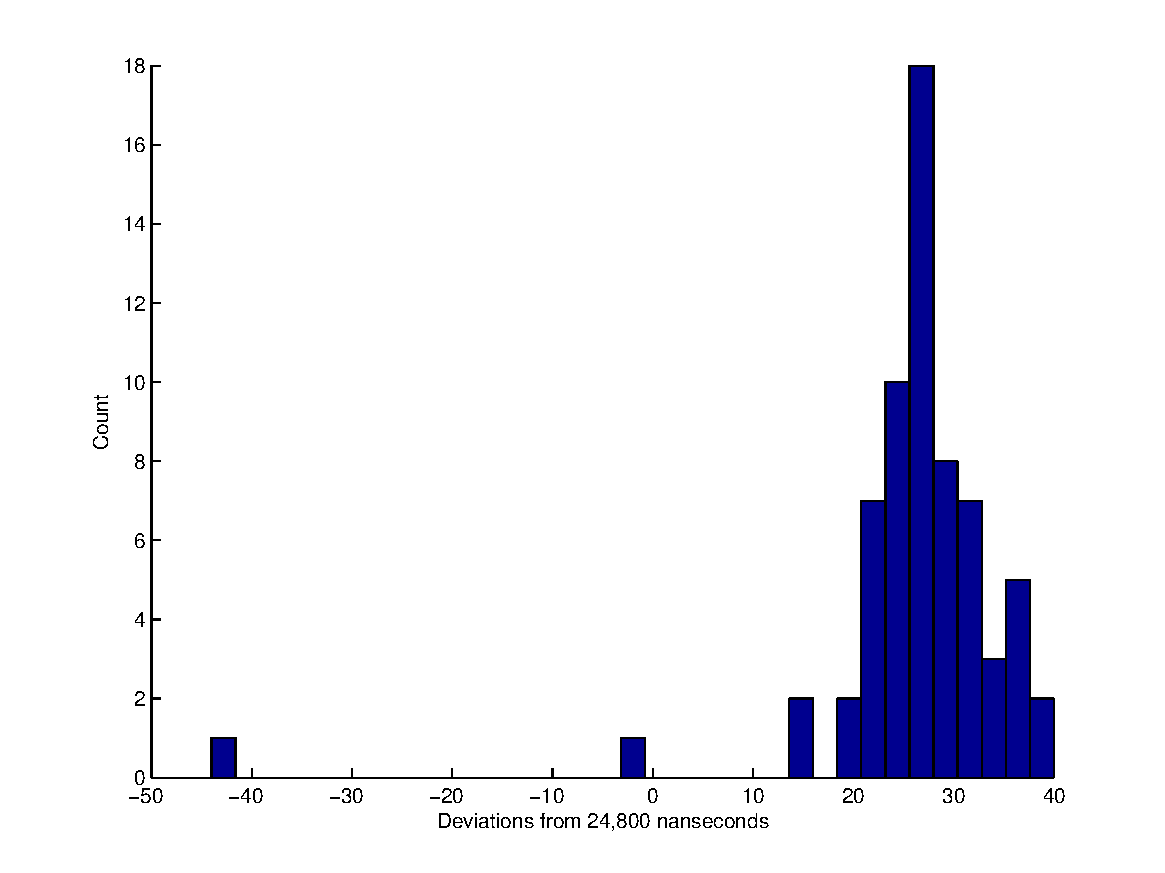
\includegraphics[width=0.32\columnwidth]{figures/newcomb_hist}
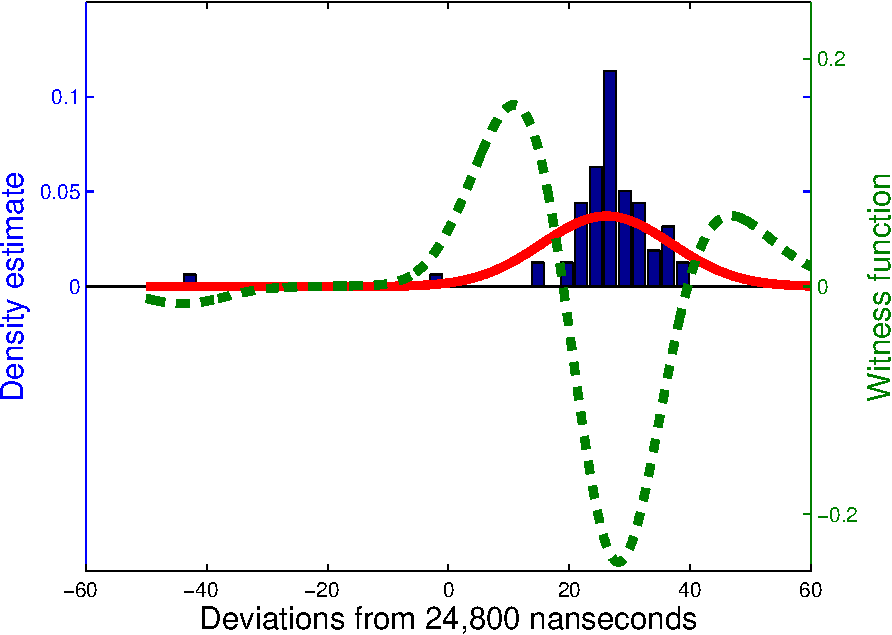
\includegraphics[width=0.32\columnwidth]{figures/newcomb_witness_1}
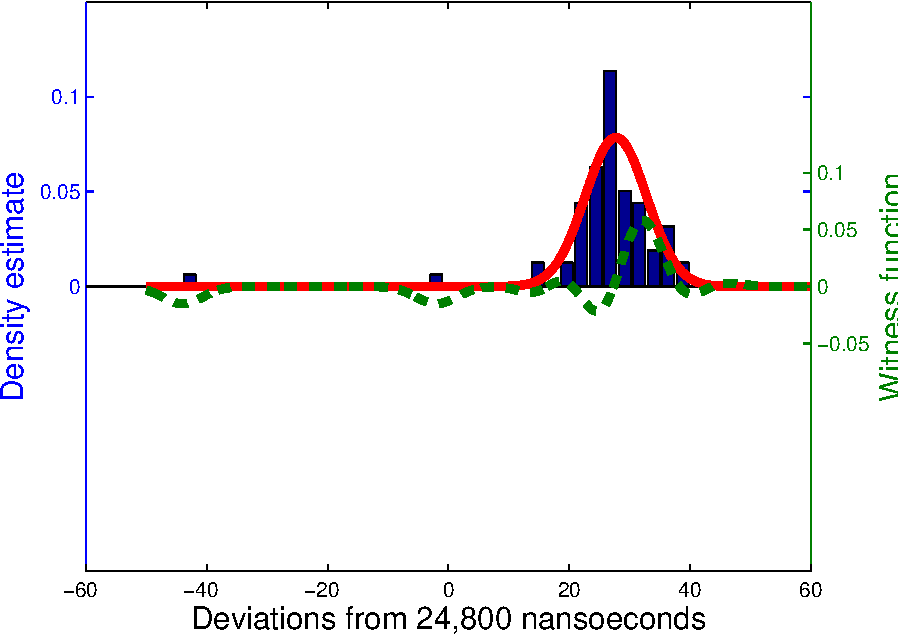
\includegraphics[width=0.32\columnwidth]{figures/newcomb_witness_2}
\caption{
Left: Histogram of Simon Newcomb's speed of light measurements.
Middle: Histogram together with density estimate (red solid line) and MMD witness function (green dashed line).
Right: Histogram together with improved density estimate witness function.
}
\label{fig:newcomb}
\end{figure}

To perform a MMD two sample test we sampled 1000 points from the fitted distribution, used the median heuristic to select a lengthscale and estimated the null distribution using 1000 bootstrap replications.
The estimated $p$-value of the test was less than 0.001 \ie a clear disparity between the model and data.
The data, fitted density estimate (the normal distribution) and witness function are shown in the middle of figure~\ref{fig:newcomb}.
The witness function has a trough at the centre of the data and peaks either side.
This indicates that the fitted model has placed too little mass in its centre and too much mass outside its centre.
We can therefore speculate that the data is more leptokurtic (has heavier tails) than the fitted model.

This suggests that we should modify our model by either using a distribution with heavy tails or explicitly modelling the possibility of outliers which could have resulted in the variance being over-estimated.
However, to demonstrate some of the properties of the MMD statistic we make an unusual choice of fitting a Gaussian by maximum likelihood, but ignoring the two outliers in the data.
The new fitted density estimate (the normal distribution) and witness function of an MMD test are shown on the right of figure~\ref{fig:newcomb}.
The estimated $p$-value associated with the MMD two sample test is roughly 0.5, despite the fitted model being a very poor explanation of the outliers.
This demonstrates that the MMD test using a radial basis function kernel identifies dense discrepancies, rather than outliers.
However, methods that are not robust to outliers (\eg fitting a Gaussian by maximum likelihood) will likely show dense discrepancies that will be identified by the test.

%\subsection{Spotting an unusual cluster}
%
%Figure~\ref{fig:blob_blob_ring} shows synthetic 2 dimensional data generated from two Gaussians and a uniform ring density (green circles).
%
%\begin{figure}[ht]
%\centering
%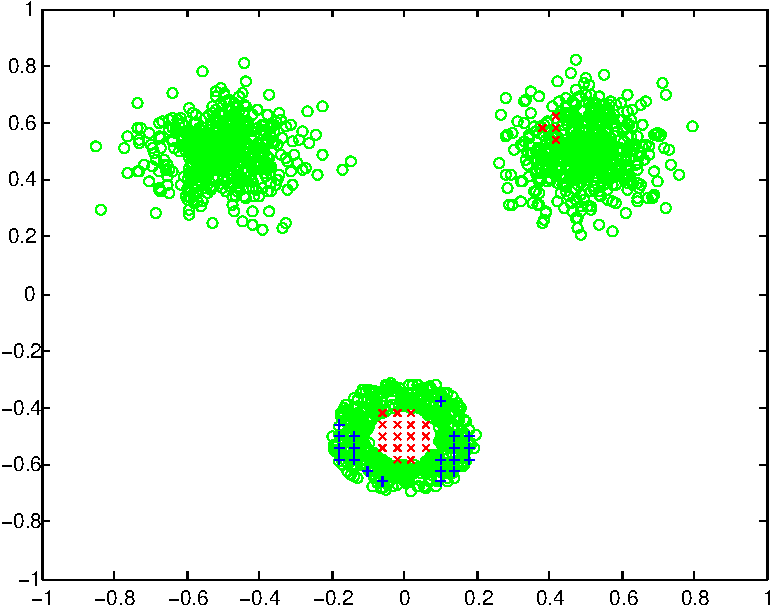
\includegraphics[width=0.98\columnwidth]{figures/blob_blob_ring}
%\caption{
%An experiment on synthetic data revealing a statistically significant maximum mean discrepancy.
%Green $\circ$ are data, red $\times$ are locations over-represented by the model, blue $+$ are locations under-represented by the model.
%}
%\label{fig:blob_blob_ring}
%\end{figure}
%
%We fit a mixture of Gaussians (cite) to this data using 3 centres.
%The kernel two sample test using the median lengthscale heuristic returns a $p$-value of (insert number here) indicating that no discrepancies can be identifed at this lengthscale.
%However, plotting a histogram of all pairwise distances over the data reveals two predominant scales in the data; the median is closest to the larger value.
%
%Performing a kernel two sample test with the smaller lengthscale results in a $p$-value of (insert number) indicating a discrepancy between the model and the data.
%Similar to before we can identify this discrepancy via the witness function.
%\TBD{
%Something about extreme points or basins of attraction or a plot of the witness function.
%}
%The witness function has clearly identified the uniform ring of data points as being inconsistent with the mixture of Gaussians model.
%
%\TBD{Follow up could be trying to fit this with more Gaussians - how many do we need to patch it up - will there always be discrepancies or will they become too small to notice?}

\subsection{High dimensional data}

\label{sec:high_dim}

The interpretability of the witness functions comes from being equal to the difference of two kernel density estimates.
In high dimensional spaces, kernel density estimation is a very high variance procedure that can result in poor density estimates\fTBD{what is a classic citation?} which will destroy the interpretability of the method.
In response, we consider using dimensionality reduction techniques\fTBD{what is a classic citation?} before performing two sample tests.
Note however that the statistical test derived from the MMD still has high power in high dimensions \citep{Gretton2008-ik}.

To test how the MMD statistic can be used for high dimensional data we generated synthetic data using the following recipe.
5 points in a 10 dimensional space were drawn at random from a random 4 dimensional subspace\footnotemark.
\footnotetext{The details are not especially important; code for replication will be available upon publication}
Data was generated as isotropic Gaussian distributions centred on 4 of the 5 points.
Finally, data was centred on the fifth point drawn from an isotropic $t$-distribution with 2 degrees of freedom.
In sum, the data is a mixture of Gaussians and a $t$-distribution.

We then fit a mixture of Gaussians\fTBD{what is a classic citation?} with 5 centres to the data and then generated samples from the fitted distribution in order to perform an MMD two sample test.
We reduced the dimensionality of the data using principal component analysis (PCA), selecting the first two principal components.
To ensure that the MMD test remains well calibrated we include the PCA dimensionality reduction within the bootstrap estimation of the null distribution.
The data and posterior predictive samples are plotted on the left of figure~\ref{fig:high_mog}.
While we can see that one cluster is different from the rest, it is difficult to assess by eye if these distributions are different due in part to the difficulty of plotting two sets of samples on top of each other.

\begin{figure}[ht]
\centering
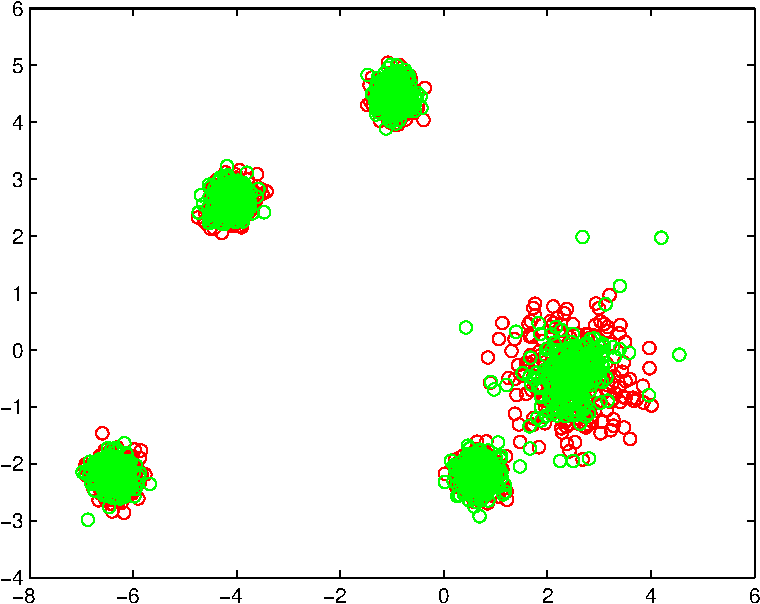
\includegraphics[width=0.4\columnwidth]{figures/high_mog_pca}
\hspace{0.1\columnwidth}
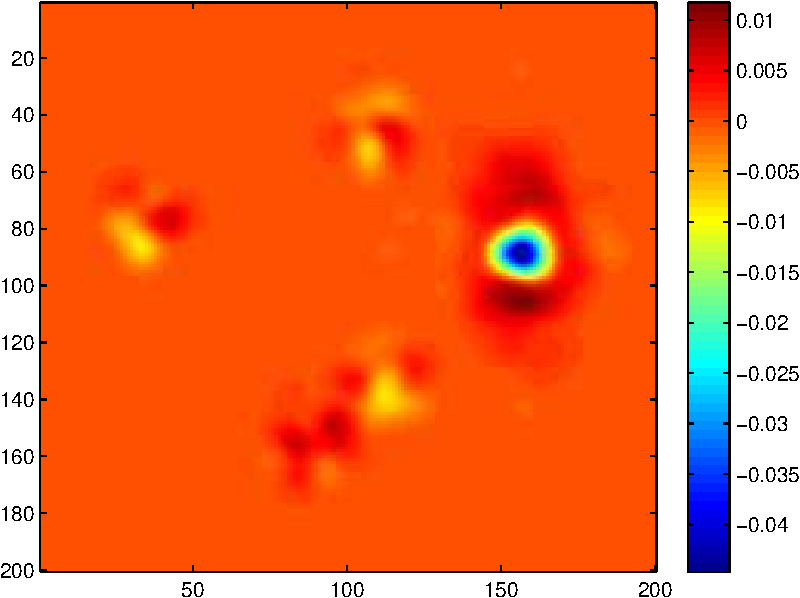
\includegraphics[width=0.4\columnwidth]{figures/high_mog_witness}
\caption{
Left: PCA projection of synthetic high dimensional cluster data (green circles) and projection of samples from fitted model (red circles).
Right: Witness function of MMD two sample test. The erroneously fit cluster is clearly identified.
}
\label{fig:high_mog}
\end{figure}

Using the median heuristic to select a lengthscale results in a test that returns a $p$-value of 0.91, indicating that the test has not identified any discrepancies.
Indeed, the lengthscale chosen by this heuristic is $4.4$ which is of the order of the distances between clusters.
The test therefore is blind to discrepancies smaller than distances between clusters, and since the mixture of Gaussians has correctly identified the 5 centres and sizes of the mixture distribution, the test does not find any discrepancies.

However, taking the density estimate interpretation of the witness function more seriously suggests choosing lengthscales that result in the best density estimates.
We therefore selected a lengthscale by 5 fold cross validation using predictive likelihood of the kernel density estimate as the selection criterion.
With this lengthscale the MMD test returns a $p$-value of 0.05 and the witness function (right of figure~\ref{fig:high_mog}) clearly identifies the cluster that has been incorrectly modelled.

Presented with this discrepancy a statistical modeller might try a more flexible clustering model \citep{Peel2000-pv, Iwata2012-yj} (a mixture of $t$-distributions would work on this example).
However, the $p$-value of the MMD statistic can also be made non-significant by fitting a mixture of 10 Gaussians.
We mention this as a reminder that the test proposed here does not assess the `truth' of a model, only whether the data could plausibly have been generated by the model.

\section{Applications to real data and complex statistical models}

\subsection{What exactly do neural networks dream about?}

``To recognize shapes, first learn to generate images'' quoth Hinton \citep{Hinton2007-eo}.
Restricted Boltzmann Machine (RBM) pretraining of neural networks was shown by \cite{Hinton2006-yw} to learn a deep belief network (DBN)\fTBD{What is a canononical reference?} for the training data \ie a generative model.
Subsequently, as well as computing estimates of marginal likelihoods and testing errors, it became standard to demonstrate the effectiveness of a neural network by generating samples from the distribution it had learned\fTBD{cite things}.

When trained on the MNIST handwritten digit data, the samples certainly look like digits, but it is hard to detect any systematic anomalies purely by visual inspection.
We now use the kernel MMD two-sample test to investigate how faithfully RBMs and DBNs can capture the probability distribution over handwritten digits.

\subsubsection{RBMs mistake the identity of digits}

We trained an RBM with architecture $(784)\leftrightarrow(500)\leftrightarrow(10)$\footnotemark~using 15 epochs of persistent contrastive divergence PCD-15 (\NA{cite something}), a batch size of 20 and a learning rate of 0.1 (\ie we used the same settings as the code available at \NA{cite deep learning tutorial}).
\footnotetext{That is, 784 input pixels and 10 indicators of the class label are connected to 500 hidden neurons.}
We generated 3000 independent samples from the learned generative model by initialising the network with a random training image and performing 1000 clamped gibbs updates\footnotemark~to generate each image (as in \eg \cite{Hinton2007-eo}).
\footnotetext{Without clamping the label pixels, the generative distribution is heavily biased towards certain digits.}

The top left of figure~\ref{fig:digits} shows the twenty random samples\footnotemark~from this model.
\footnotetext{
Specifically these are the activations of the pixel neurons before sampling sampling binary values.
This is an attempt to be consistent with the grayscale input distribution of the images.
Analogous discrepancies would be discovered if we had instead sampled binary pixel values.}
They certainly look mostly like digits, but has the true distribution over digits been faithfully captured?
A priori the answer to this question is almost certainly no, but it is not immediately obvious how the learned distribution will deviate from the true distribution.

\begin{figure}[ht]
\centering
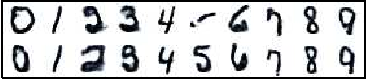
\includegraphics[width=0.48\columnwidth]{figures/rbm_samples}
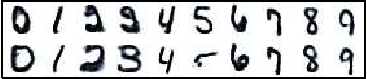
\includegraphics[width=0.48\columnwidth]{figures/rbm_witness_troughs}
\\
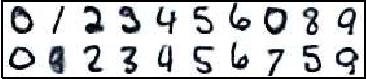
\includegraphics[width=0.48\columnwidth]{figures/many_rbm_cond_witness_troughs}
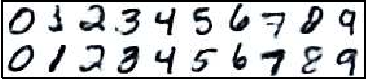
\includegraphics[width=0.48\columnwidth]{figures/dbn_ft_cond_witness_troughs}
\\
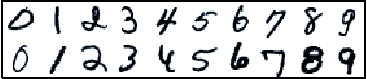
\includegraphics[width=0.48\columnwidth]{figures/many_rbm_cond_witness_peaks}
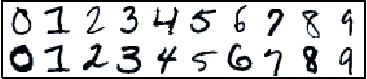
\includegraphics[width=0.48\columnwidth]{figures/dbn_ft_cond_witness_peaks}
%\\
%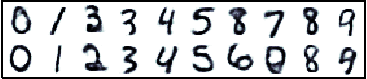
\includegraphics[width=0.48\columnwidth]{figures/many_rbm_samples}
%\includegraphics[width=0.48\columnwidth]{figures/dbn_ft_samples}
%\\
%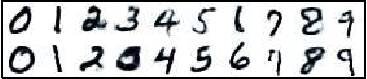
\includegraphics[width=0.48\columnwidth]{figures/dbn_ft_samples_2}
%\includegraphics[width=0.48\columnwidth]{figures/dbn_ft_samples_3}
%\\
%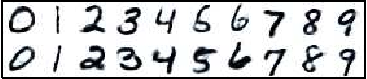
\includegraphics[width=0.48\columnwidth]{figures/dbn_ft_samples_1}
%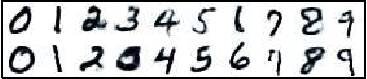
\includegraphics[width=0.48\columnwidth]{figures/dbn_ft_samples_2}
\caption{
Top left: Random samples from an RBM.
Top right: Troughs of the witness function for the RBM (digits that are over-represented by the model).
Middle left: Troughs of the witness function for samples from several RBMs.
Middle right: Troughs of the witness function for the DBN.
Bottom left: Peaks (digits that are under-represented by the model) of the witness function for samples from several RBMs.
Bottom right: Peaks of the witness function for the DBN.
}
\label{fig:digits}
\end{figure}

Since we generated digits from the class conditional distributions we compare each class separately.
Rather than show plots of the witness function for each digit we summarise the witness function by examples of digits closest to the peaks and troughs of the witness function (the witness function estimate is differentiable so we can easily find the peaks and troughs by gradient based optimisation).
We apply the MMD two-sample test to each class conditional distribution, using PCA to reduce to 2 dimensions and selecting the lengthscale via cross validation as in section~\ref{sec:high_dim}.

The top right box of figure~\ref{fig:digits} shows the digits closest to the two most extreme troughs\footnotemark~of the witness function for each class; the troughs indicate where the fitted distribution over-represents the distribution of true digits.
\footnotetext{
The exact ordering of the peaks and troughs is as follows.
We partition the space by grouping samples where the witness function has the same sign and gradient based optimisation of the witness function starting from each sample would reach the same peak or trough.
The contribution of the MMD from each of these groups is used to order the peaks and troughs.
}
The estimated $p$-value for all tests was less than 0.001.
The most obvious error with these digits is that the first 2s and 3s look quite similar.

To test that this was not just a poorly trained single RBM, we trained 1500 RBMs (with differently initialised pseudo random number generators) and generated one sample from each and performed the same tests.
The estimated $p$-values were [something - significant] and the summaries of the troughs of the witness function are shown in the middle left box of figure~\ref{fig:digits}.
On the first toy data example we observed that the MMD statistic does not highlight outliers and therefore we can conclude that RBMs are making consistent mistakes \eg generating a 0 from the 7 distribution or a 5 when it should have been generating an 8.\fTBD{Do we want to try to say more? Speculate why?}

\subsubsection{DBNs have nightmares about ghosts}

We now test the effectiveness of deep learning to represent the distribution of MNIST digits.
In particular, we fit a DBN with architecture $(784)\leftarrow(500)\leftarrow(500)\leftrightarrow(2000)\leftrightarrow(10)$ using RBM pre-training and a generative fine tuning algorithm proposed in (\NA{cite Geoff again}).
Performing the same tests with 3000 samples results in estimated $p$-values of less than 0.001 except for the digit 4 (0.150) and digit 7 (0.01).
Summaries of the witness function troughs are shown in the middle right box of figure~\ref{fig:digits}.

The witness function no longer shows any class label mistakes (except perhaps for the digit 1 which looks very peculiar) but the 2, 3, 7 and 8 appear `ghosted' \ie the digits fade in and out.
For comparison the bottom right box of figure~\ref{fig:digits} shows digits closest to the peaks of the witness function; there is no trace of ghosting.

Returning to the RBMs, we do not see ghosting, but the digits nearest the witness function troughs are somewhat blurred (see bottom left box for comparison with peaks).
Assuming that the top level associative memory of the DBN also suffers from blurring, this will result in occasionally incorrect neurons in the second hidden layer on the DBN.
These incorrect bits will then propagate down the DBN resulting in spurious features in several visible neurons, resulting in ghosting.

\TBD{
Speculate on fixes.
Thresholding of some sort?
Do we discuss whether or not this could have been concluded without the tests?
Different architectures to discourage mistakes from propagating?
}

\subsection{Something about LDA}

\TBD{Something about LDA}

\section{Discussion of model criticism and related work}

\subsection{Are we criticising a particular model, or class of models?}

To a frequentist, a statistical model is typically a probability distribution over data with some unknown parameters.
To a Bayesian, the specification of a model is only complete with a prior distribution for those parameters.
This difference in terminology is perhaps behind some of the confusion in the literature about the validity of certain model criticism techniques which we now discuss.

Posterior predictive $p$-values and the test proposed here test the null hypothesis that the data was generated from a particular probability distribution - a model with fitted parameters or the posterior predictive distribution.
These tests allow us to falsify the hypothesis that a fitted model or posterior predictive distribution is a faithful summary of the data.
Note however that some proponents of posterior predictive $p$-values prefer to interpret them directly as subjective Bayesian probabilities \citep{Gelman2013-am}.

A more classical null hypothesis associated with model criticism is that the data was generated from a probability distribution of a certain form but with unknown parameters (\eg all normal distributions).
Posterior $p$-values are uncalibrated for this composite hypothesis test \citep{Robins2000-oz} - under broad assumptions posterior predictive $p$-values are asymptotically conservative (the null distribution is concentrated towards values of 0.5).
Robins et alia \citep{Robins2000-oz} shows that alternatives proposed by Bayarri \& Berger \citep{Bayarri1999-ty}, and prior predictive $p$-values of Box \citep{Box1980-ud} among others are appropriately calibrated.
Further examples of tests that are calibrated for this composite null hypothesis incude \citep[e.g.][]{Dey1998-dn, Johnson2004-ej}

However, in our first real data example we are not interested in the question `do MNIST digits come from some deep belief network?'.
If we were trying to answer this question, then we should expect any calibrated $p$-value to have very low statistical power since the space of probability distributions that can be represented by a deep belief network is very large indeed.
Insead it is of more interest for this example to ask whether or not our particular neural network can faithfully mimick the distribution it was trained on.

\subsection{When can we ignore a discrepancy between a model and data?}

The test proposed in this paper indicates whether or not it is plausible that the data was generated by a fitted model or posterior distribution.
A significant value of the test statistic does not always indicate that the model was in some sense defective.
For example, if one had a very strong prior on some model parameter for rational reasons, but that differed from the true generating process, it would take a lot of data for one's posterior distribution to converge to the distribution from which the data was being generated.
Consequently, the MMD statistic would have a significant value for many sizes of data, but this would be accurately indicating that the posterior distribution is likely to be a poor description of the true data generation process.

In light of this observation the test proposed here may be most appropriate when trying to perform a Bayesian analysis that uses reference priors\fTBD{I need to find a reference} where the priors are chosen to minimise the impact on the posterior, or when one has a large quantity of data.
However, we believe it is still of value to know when one's posterior belief differs from observed data, even if this may be entirely reasonable from a subjective viewpoint.

\subsection{Should we worry about using the same data for traning and criticism?}

The test proposed here attempts to falsify the null hypothesis that the data could have been generated by the fitted model or posterior predictive distribution.
In some situations it may be more appropriate to attempt to falsify the the null hypothesis that future data will be generated by the posterior predictive distribution.
This can be achieved by reserving a portion of the data to be used for model criticism alone, rather than fitting a model or updating a posterior on the full data.
Cross validation methods have also been investigated in this context \citep{Gelfand1992-ow, Gelfand1996-vy, Marshall2007-hd}

\subsection{Omnibus methods for model criticism}

Gelman, Meng \& Stern \citep{Gelman1996-ez} proposed an extension to posterior predictive $p$-values of Rubin \citep{Rubin1984-tw} by generalising the test statistic to a discrepancy meansure that can also take model parameters as input as well as data.
In doing so they also proposed an omnibus test discrepancy measure
\begin{equation}
  X^2(y,\theta) = \sum_{i=1}^n \frac{(y_i-\mathbb{E}(y_i\given\theta))^2}{\textrm{Var}(y_i\given\theta)}
\end{equation}
which resembles a classical $\chi^2$ statistic.
While this statistic can be useful in a number of different models, regression models especially, it would have failed to detect any discrepancies in our two toy data examples.
In the case of exchangeable data (and a model that respects this symmetry) this statistic only measures how well the mean and variance of the data has been captured.
In our two toy data examples the mean and variance of the data were fit (near) directly by the proposed models.\fTBD{Check that this statement is true}

\subsection{Other methods for evaluating statistical models}

Other typical methods of model evaluation include estimating the predictive performance of the model, analyses of sensitivities to modelling parameters / priors, graphical tests, and estimates of model utility.
For a recent survey of Bayesian methods for model assessment, selection and comparison see \cite{Vehtari2012-oh} which phrases many techniques as estimates of the utility of a model.
For some discussion of sensitivity analysis and graphical model comparison see \citep[e.g.][]{Gelman2013-st}.

O'Hagan \citep{OHagan2003-bc} considers using Kullback-Leibler divergences between prior and posterior distributions in hierarchical models.

In the spirit of scientific falsification\fTBD{A canonical Popper reference?}, ideally all methods of assessing a model should be performed to gain confidence in any conclusions made.

\section{Conclusions and future work}

In this paper we have demonstrated an exploratory form of model criticism based on two sample tests using kernel maximum mean discrepancy.
In contrast to other methods for model criticism, the test analytically maximises over a broad class of statistics, automatically identifying the statistic which most demonstrates the discrepancy between the model and data.
We demonstrated how this method of model criticism can be applied to neural networks and \NA{something else} and demonstrated the ways in which these models were misrepresenting the data they were trained on.

We have demonstrated how kernel MMD two sample tests can be applied to model criticism, but they can be applied to any aspect of statistical modelling where two sample tests are useful.
This includes for example, Geweke's tests of markov chain posterior sampler validity \citep{Geweke2004-yx} and tests of markov chain convergence\fTBD{I presume this is a thing?}.

The two sample tests proposed in this paper apply to exchangeable data, but model criticism techniques should of course apply to models with other symmetries (\eg logitudinal data, graphs, functions\ldots).
While two sample tests exist for data with different symmetries (\NA{cite something related to functional two sample testing}) it is unclear whether maximum mean discrepancy measures can be naturally extended to these classes; investigating such extensions would be a profitable area for future study.

\TBD{Repeat of the call to arms about a lack of model checking in machine learning. Do you know what your model is up to right now? Maybe you should check it is ok.}

\newpage

\bibliography{experiment}
\bibliographystyle{unsrt}

\end{document} 

%%%%%%%%%%%%%%%%%%%%%%%%%%%%%
%%%%%%%%%%%%%%%%%%%%%%%%%%%%%

\subsubsection{Alternative maths}

\TBD{This is probably superfluous and not helpful?}

To demonstrate the connection between posterior predictive $p$-values and maximum mean discrepancy measures we rewrite the $p$-value as an expectation
\begin{equation}
\mathbb{E}(\mathbb{I}[T(Y^\textrm{rep}) - T(Y) > 0]).
\end{equation}
We now remove the indicator function from this expression
\begin{equation}
  \mathbb{E}(T(Y^\textrm{rep})) - T(Y)
\end{equation}
yielding a measure of how the posterior mean of the statistic compares to the statistic evaluated on the data.
If we assume that our statistic $T$ is of the form $T(Y) = \sum t(y_i)$ (this includes \eg all empirical moments) then
\begin{equation}
\mathbb{E}(T(Y^\textrm{rep})) - T(Y) = \sum \mathbb{E}(t(y_i^\textrm{rep})) - \sum t(y_i) = \mathbb{E}(t(y^\textrm{rep})) - \mathbb{E}(t(y))
\end{equation}
where $y$ and $y^\textrm{rep}$ are distributed according to the empirical distribution of the data and the posterior-predictive distribution over single data points respectively.
This quantity is called a mean discrepancy between the distribution of $y$ and $y^\textrm{rep}$.

In the practical application of posterior-predictive $p$-values, statistics are chosen to measure aspects of the data that are of relevance to the analysis being performed.
Whilst there are numerous examples (\NA{cite some applied papers}) of sensible choices for standard models, there is little work on exploratory model checking.
The benefit of considering mean discrepancies is that we can analytically maximise over a large space of different statistics.

\TBD{
Can we relate any of this to utility theory.
Using scoring rules to justify the use of the posterior predictive.
}

\subsubsection{Alternative maths}

In this setting it is natural to replace the posterior predictive distribution over data sets with the posterior predictive distribution over data points
\begin{equation}
p(y^\textrm{rep}|M,Y) = \int p(y^\textrm{rep}|M,\theta)p(\theta|M,Y)\mathrm{d}\theta.
\end{equation}
We then define posterior predictive $p$-values as
\begin{equation}
  p_\textrm{x}(Y) = \mathbb{P}_{y\sim \hat{Y}}(T(y^\textrm{rep})\geq T(y)|M,Y) = \mathbb{E}_{y\sim \hat{Y}}(\mathbb{I}[T(y^\textrm{rep}) - T(y) > 0])
\end{equation}
where $\hat{Y}$ if the empirical distribution of the data.
This is a measure of how extreme the data is compared to the posterior predictive distribution over data points.
If we remove the indicator function in the above equation we get
\begin{equation}
  \mathbb{E}(T(y^\textrm{rep})) - \mathbb{E}(T(y))
\end{equation}
which measures the mean discrepancy between the posterior predictive distribution and the data as measured by the statistic $T$.
